%\chapter{UnBBayes}%
O UnBBayes é a ferramenta que expandiremos ao longo dos próximos semestres para desenvolver novos algoritmos.
UnBBayes é uma aplicação open-source feita em Java\texttrademark\ desenvolvido pelo \gls{gia} do Departamento de Ciência da Computação da \gls{unb} no Brasil e provê um framework para construir modelos gráficos probabilísticos e realizar raciocínios plausíveis. Ele apresenta uma \gls{gui}, \gls{api} e ainda suporte a plug-ins para extensões não previstas.

\cite{javaApi11} descreve os três objetivos principais das mais novas versões do UnBBayes, são eles:
\begin{itemize}
	\item Ser uma plataforma para a disseminação dos conceitos e utilidade do raciocínio probabilístico;
	\item Ser uma ferramenta visual fácil de usar e configurar;
	\item Fornecer extensibilidade.
\end{itemize}
O Primeiro objetivo é atingido com a implementação do estado da arte de \gls{bn} e um algoritmo de inferência padrão baseado no algoritmo de Junction Trees. O segundo através de uma a implementação de GUI intuitiva. E a terceira através da natureza orientada a objetos do Java\texttrademark\ em conjunto com um design de plug-ins.

O projeto oferece um repositório que incluem plug-ins para \gls{bn}, \gls{id}, \gls{msbn}, \gls{mebn}, \gls{prowl}, aprendizado de parametros, aprendizado de estrutura e aprendizado incremental de \glspl{bn}, data mining, avaliação de classificação e perfomance e análise estatística de dados e finalmente diversos algoritmos para inferencia Bayesiana. A Figura \ref{fig:unbbayes_usage} ilustra um diagrama de caso de uso do UnBBayes core\footnote{O core é uma aplicação com um mínimo de funcionalidades.}.

\begin{figure}[H]
	\centering
	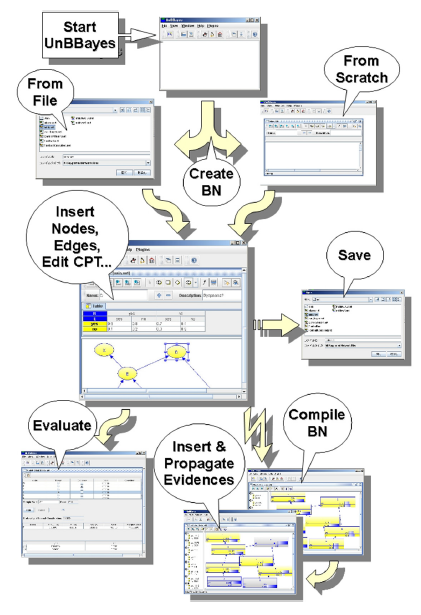
\includegraphics{figuras/unbbayes_usage}
	\caption[Diagrama de uso do UnBBayes]{Um exemplo de diagrama de uso do UnBBayes core (módulo de \gls{bn} e da \gls{gui} (Retirado de...)}
	\label{fig:unbbayes_usage}
\end{figure}


\section{Design Geral}
O UnBBayes é basicamente estruturado no design pattern \gls{mvc}
(ver capítulo 6).

A Figura \ref{fig:unbbayes_mvc} ilustra o design geral do UnBBayes.
\begin{figure}[H]
	\centering
	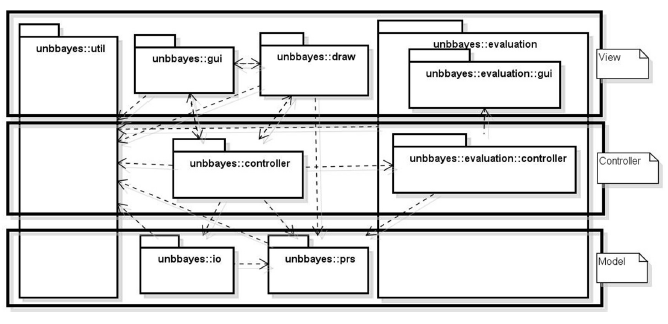
\includegraphics[width = 440px]{figuras/unbbayes_mvc}
	\caption[UnBBayes UML MVC]{uma classe UML ilustrando o design MVC do UnBBayes, em nível de pacotes. (Retirado de \cite{javaApi11})}
	\label{fig:unbbayes_mvc}
\end{figure}

Apesar do UnBBayes ser escrito em Java\texttrademark\, que é uma linguagem tipicamente \gls{oo}, o UnBBayes raramente aplica uma orientação a objetos pura em seu design. Mas ao invés, ela segue uma adaptação do paradigma orientado a componentes, o qual organiza os pedaços de código em conjuntos destacáveis e substituíveis. Componentes como num circuito eletrônico, como por exemplo circuitos integrados.

Designs baseados em componentes provêem uma alta variabilidade e reusabilidaide, o que são alguns dos grandes requerimentos mencionados na seção anterior. Isto porque para fazer modificações no programa, basta substituir aquele componente por um outro. Por exemplo se precisarmos trocar o formato de um nó basta substituir o objeto que o rederiza. O que significa dizer que não há necessidade de entrar dentro de uma classe já pronta e configurar aquelas linhas de código.

O módulo core do UnBBayes provê duas funcionalidades mestras: a infraestrutura base (por exemplo, suporte às telas, acesso aos arquivos, suporte a plug-ins) e uma manipulação de \gls{bn} com funcionalidades básicas (por exemplo inferência e manipulação). A seguir listamos os pacotes que compõem o core (a Figura \ref{fig:unbbayes_mvc} apresentou suas dependências gerais).

\begin{itemize}
	\item unbbayes.controller: Contem as classes do controller do MVC
%	it contains controller classes of MVC model.
	
	\item unbbayes.draw: Contem os adapters para determinar como um grafo é desenhado na tela. Permite diversas funcionalidades para desenhar, incluindo redimencionar, colorir, mover, etc.
	
	\item unbbayes.evaluation: Contém classes para estimar a \gls{bn}
	

	\item unbbayes.gui: contem as Classes das \gls{gui} (por exemplo panels, windows, forms, tables).
	
	\item unbbayes.io: contem classes para armazenamento de \gls{bn}, configurações, preferencias, logs como arquivos.

	\item unbbayes.prs: contem classes representando estrutura de dados e algoritmos (classes da model do MVC.) Elementos conceituais (Node, Edge, Network, JunctionTree, PotentialTable) e as operações entre eles . PRS vem de Probabilistic Reasoning System, isto é, o sistema de raciocinio probabilistico. Classes nesse pacote representam a \gls{bn}, classes no unbbayes.prs.id representa uma \gls{id}, e classes no unbbayes.prs.hubrdbn representa uma hybrid \gls{bn}, que inclui nós contínuos com valor númerico.

	\item unbbayes.example: contem classes exemplificando o uso da API do UnBBayes.

	\item unbbayes.util: este pacote unifica as classes de utilidade, os quais são classes de propósito gerais utilizados. Classes colocadas aqui provêm as seguintes funcionalidades: debugging, classes abstratas para design patterns e manipulação de coleções avançadas.
	
	\item *.resources: pacotes com este padrão de nome contêm classes de recursos, os quais provêem funcionalidade de lcalização. O class loader32 do UnBBayes  pode selecionar as classes de recursos apropriados automaticamente, dependendo das configurações do computador.

	\item *.extension: pacotes com esse padrão de nome contêm classes implementando funcionalidades relacionadas à infra-estrutura de plug-in.

	\item *.exception: pacotes com esse padrão de nome contem classes representando classes de excessão.
\end{itemize}

\subsection{Classes da View e Controller}
A lista a seguir oferece uma breve descrição das classes ilustradas na Figura \ref{fig:unbbayes_viewcontrol}
\begin{itemize}
	\item NamedWindowBuilder: este é um builder que instancia uma janela interna. Cada janela instanciada por estes builders terão um identificador (nome) e será colocado no MDIDesktopPane. Esta classe elimina dependencia direta do MainController às classes do módulo de \gls{bn} (por exemplo NetworkWindow)

	\item NetworkWindowBuilder: a builder para NetworkWindow
	
	\item MainController: este é o controlador responsável por criar, carregar e salvar redes que o UnBBayes suporta. Também lida com as configurações de sistema.
	
	\item UnBBayesFrame: esta é uma extensão do swing JFrame responsável pelo painel principal do UnBBayes.
	
	\item MDIDesktopPane: Esta é uma extensão do swing JDesktopPane e oferece suporte à funcionalidade \gls{mdi} (isto é, multiplas janelas dentro de uma janela pai). Esta classe também lidai com as barras de scroll para quando a janela interna move muito para a direita ou para baixo da janela principal.
	
	\item NetworkController: este é o controlador responsável por engatilhar as operações do módulo de \gls{bn} (tais como inserção de nós e propagação de evidências).

	\item NetworkWindow: esta é o frame interno onde a edição de \gls{bn} é feita.

	\item PNCompilationPane: este é o painel da NetworkWindow responsável por mostrar a \gls{bn} compilada e oferecer os meios para inserir e propagar evidências.
	
	\item GraphPane: este é o painel da NetworkWindow responsável por mostrar a representação gráfica da \gls{bn} sendo editada.

	\item PNEditionPane: este é um painel na NetworkWindow responsável por prover as ferramentas para edição da \gls{bn}
	
	\item UShape: esta classe é responsável por renderizar os nós em um canvas. Encapsulando a classe da model Node.

	\item UCanvas: esta classe representa o canvas onde o grafo é pintado.

	\item UShapeLine: esta classe é responsável por renderaziar os arcos no canvas. Ecapsulando a classe da model Edge.
\end{itemize}

\begin{figure}[ht]
	\centering
	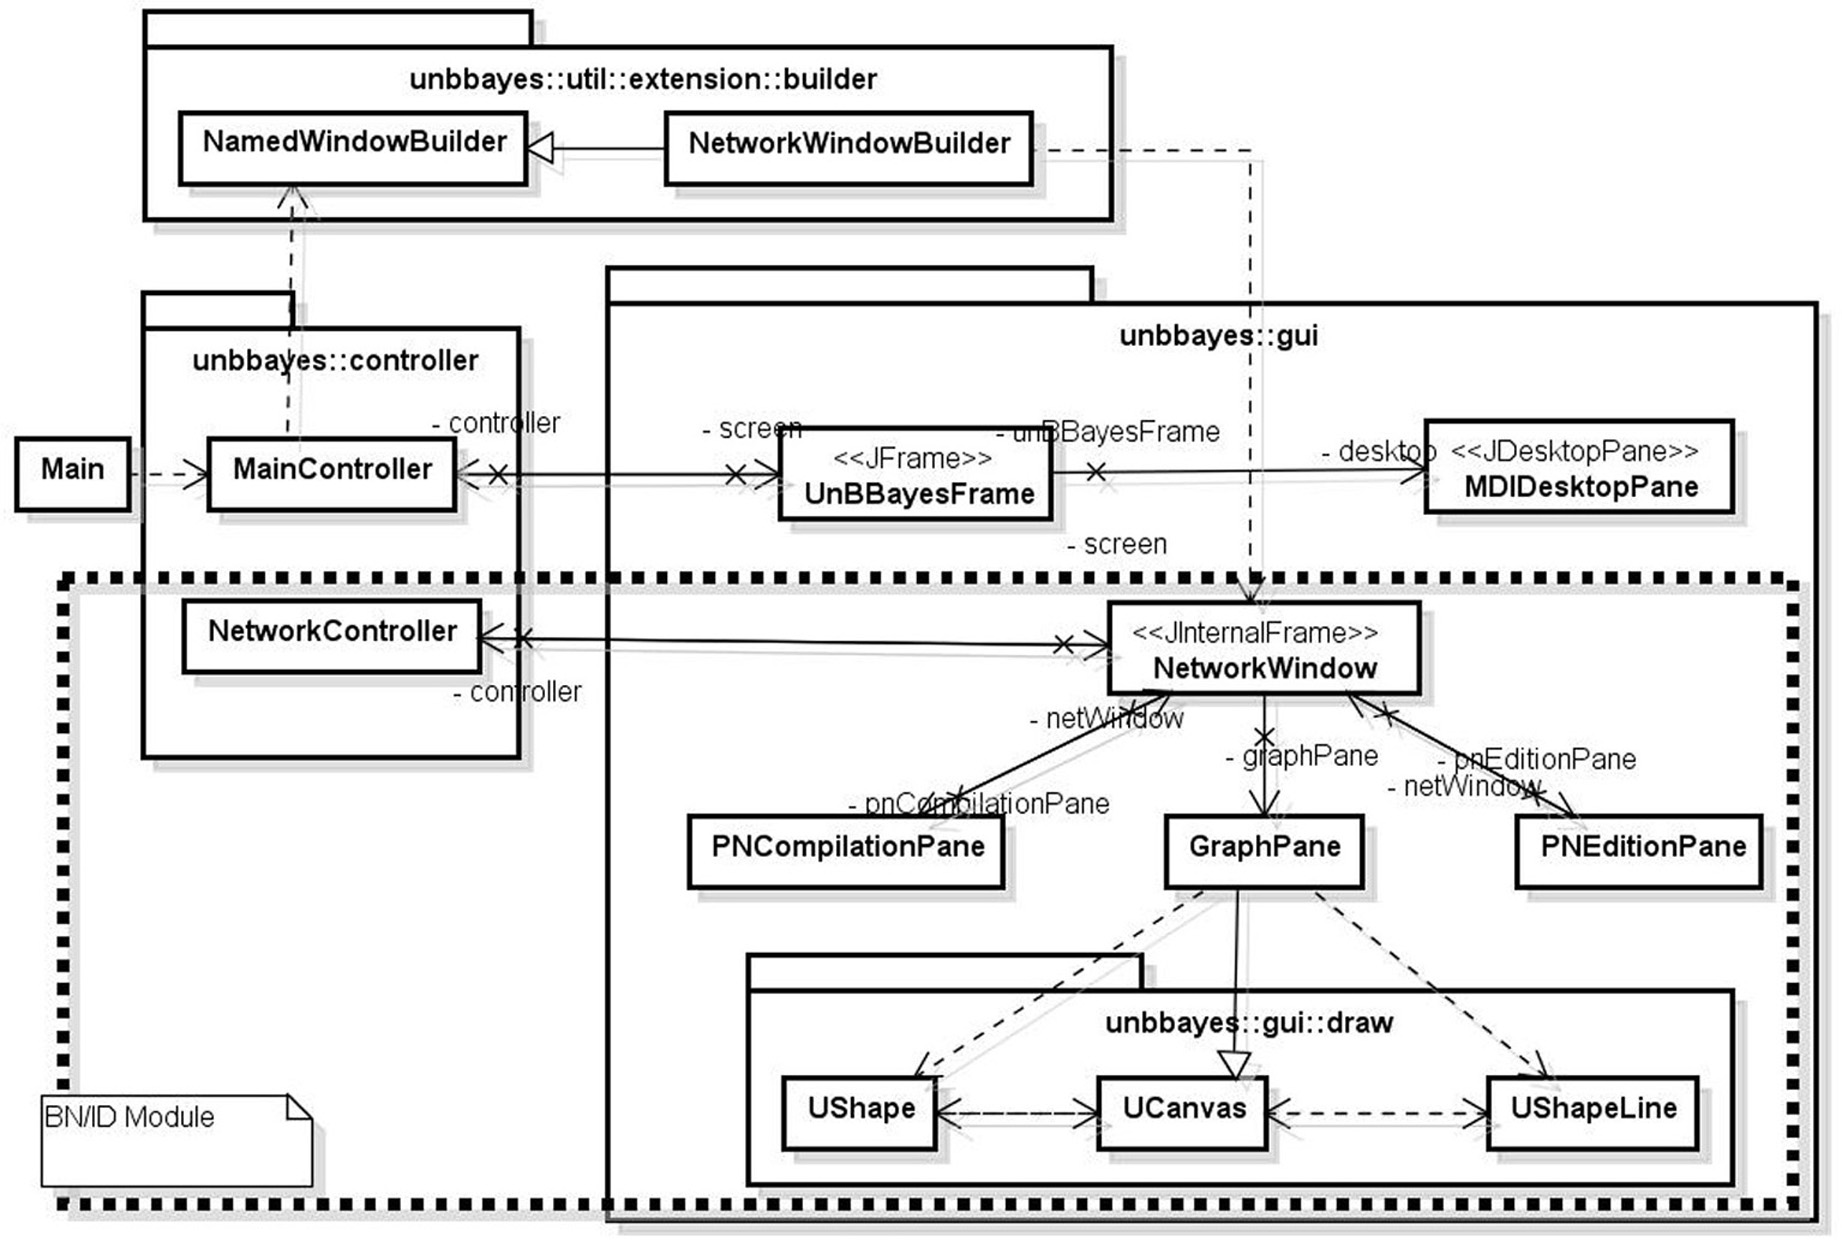
\includegraphics[width = 450px]{figuras/unbbayes_viewcontrol}
	\caption[UnBBayes View e Controller]{Classes do UnBBayes (core) implementando a View e o Controller do MVC (Retirado de \cite{javaApi11})}
	\label{fig:unbbayes_viewcontrol}
\end{figure}

\subsection{Classes da Model}
Classes desta categoria representam dados dentro da memoria. A lista a seguir oferece uma breve descrição das classes da Figura \ref{fig:unbbayes_model}:
\begin{figure}[ht]
	\centering
	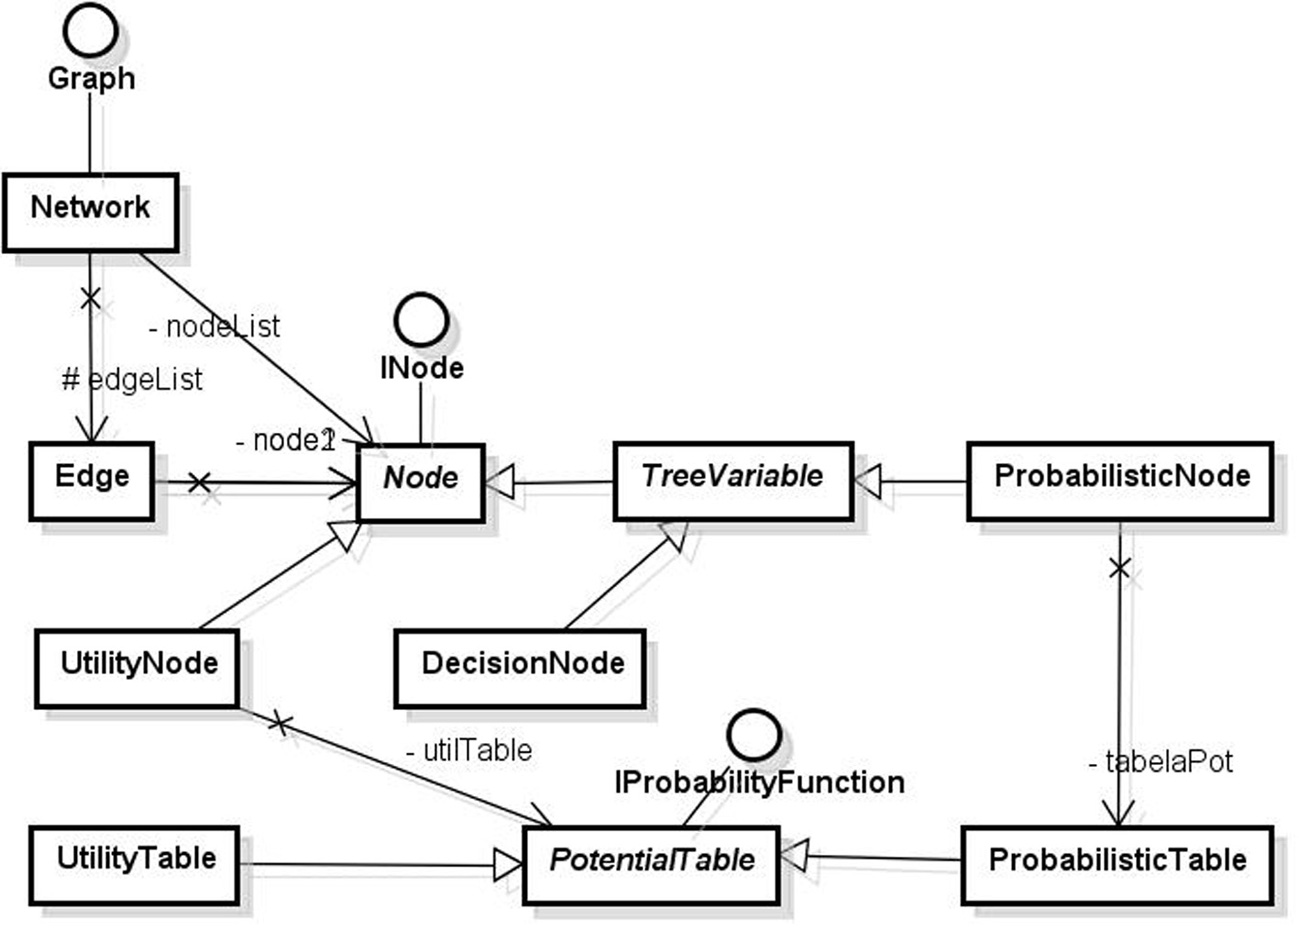
\includegraphics[width = 400px]{figuras/unbbayes_model}
	\caption[UnBBayes UML MVC]{Classes do UnBBayes (core) implementando o Model (tipo de dados e operações) do MVC (Retirado de \cite{javaApi11})}
	\label{fig:unbbayes_model}
\end{figure}

\begin{itemize}
	\item Graph: common interface for a graph built on a set of nodes and edges
	
	\item Network: concrete implementation of a generic network. If a network is composed of probabilistic nodes,
	using a ProbabilisticNetwork (an extension of Network) would be useful.
	
	\item Edge: this is a class representing an edge between two nodes. By modeling relationships as a separate
	class, it becomes possible to use attributes, thus allowing differential treatment by other classes (e.g. how
	the GUI should display a relationship between two nodes depending on the edge’s attributes). Technically,
	it is possible to create relationships (dependencies) between instances of Node without using instances of
	Edge, but in such case no arcs linking these two nodes will be rendered in the canvas. By doing so, it
	becomes possible to model “hidden” relationships.
	
	\item INode: interface representing a generic node.
	
	\item Node: abstract class representing a node. It contains additional information, such as: name, label, description,
	coordinates, flags36.
	
	\item TreeVariable: this is an abstract class for variables that will be displayed in the left side’s swing JTree
	in the compilation panel. After compiling a BN, nodes that are not extending this class will be partially
	ignored in PNCompilationPane.
	
	\item ProbabilisticNode: it represents a probabilistic node (i.e. a node having a probabilistic assignment of
	values).
	
	\item UtilityNode: this is an ID’s utility node.
	
	\item UtilityTable: this is a table representing an ID’s utility function (which is represented as a table in
	UnBBayes’ model).
	
	\item DecisionNode: this is an ID’s decision node.
	
	\item IProbabilityFunction: this is a common interface for objects specifying a node’s probabilistic distribution.
	
	\item PotentialTable: this is an abstract class representing IProbabilityFunction in a table-like format.
	
	\item ProbabilisticTable: this class represents a BN’s CPT. Objects (instances) of
	unbbayes.gui.table.GUIPotentialTable can be used to render objects of this class graphically
\end{itemize}



\section{Plugins}
Java\texttrademark\ oferece um mecanismo de fácil reuso de classes. Incorporando arquivos bytecode Java (".class" ou ".jar") no class path de outros pogramas, classes públicas e métodos serão disponibilizado ao programa como uma biblioteca. Como UnBBayes é disponibilizado como um arquivo ".jar", adicioná-lo ao class path de outro programa irá garantir acesso a sua \gls{api}.

Diferentemente de API's, plug-ins oferecem meios de rodar um novo código dentro do ambiente de execução do UnBBayes. Um plug-in é um programa que interage com a aplicação hospedeira (um core) e prover dada função. A ligação entre o plug-in e a aplicação core costuma acontecer em tempo de carregamento (quando a aplicação inicializa) ou em tempo de execução. Portanto, designs orientados a plugins oferecem ambientes práticos e flexíveis para prover variabilidade de software, uma vez que nenhuma modificação na aplicação hospedeira é necessária.
\subsection{Como desenvolver plugins}